
\documentclass[letterpaper,hide notes,xcolor={table,svgnames},pdftex,10pt]{beamer}
\def\showexamples{t}


%\usepackage[svgnames]{xcolor}

%% Demo talk
%\documentclass[letterpaper,notes=show]{beamer}

\usecolortheme{crane}
\setbeamertemplate{navigation symbols}{}

\usetheme{MyPittsburgh}
%\usetheme{Frankfurt}

%\usepackage{tipa}

\usepackage{hyperref}
\usepackage{graphicx,xspace}
\usepackage[normalem]{ulem}
\usepackage{multicol}
\usepackage{amsmath,amssymb,amsthm,graphicx,xspace}
\newcommand\SF[1]{$\bigstar$\footnote{SF: #1}}

\usepackage[default]{sourcesanspro}
\usepackage[T1]{fontenc}
\usepackage[scaled]{beramono}
\usepackage{tikzpagenodes}

\newcounter{tmpnumSlide}
\newcounter{tmpnumNote}


% old question code
%\newcommand\question[1]{{$\bigstar$ \small \onlySlide{2}{#1}}}
% \newcommand\nquestion[1]{\ifdefined \presentationonly \textcircled{?} \fi \note{\par{\Large \textbf{?}} #1}}
% \newcommand\nanswer[1]{\note{\par{\Large \textbf{A}} #1}}


 \newcommand\mnote[1]{%
   \addtocounter{tmpnumSlide}{1}
   \ifdefined\showcues {~\tiny\fbox{\arabic{tmpnumSlide}}}\fi
   \note{\setlength{\parskip}{1ex}\addtocounter{tmpnumNote}{1}\textbf{\Large \arabic{tmpnumNote}:} {#1\par}}}

\newcommand\mmnote[1]{\note{\setlength{\parskip}{1ex}#1\par}}

%\newcommand\mnote[2][]{\ifdefined\handoutwithnotes {~\tiny\fbox{#1}}\fi
% \note{\setlength{\parskip}{1ex}\textbf{\Large #1:} #2\par}}

%\newcommand\mnote[2][]{{\tiny\fbox{#1}} \note{\setlength{\parskip}{1ex}\textbf{\Large #1:} #2\par}}

\newcommand\mquestion[2]{{~\color{red}\fbox{?}}\note{\setlength{\parskip}{1ex}\par{\Large \textbf{?}} #1} \note{\setlength{\parskip}{1ex}\par{\Large \textbf{A}} #2\par}\ifdefined \presentationonly \pause \fi}

\newcommand\blackboard[1]{%
\ifdefined   \showblackboard
  {#1}
  \else {\begin{center} \fbox{\colorbox{blue!30}{%
         \begin{minipage}{.95\linewidth}%
           \hspace{\stretch{1}} Some space intentionally left blank; done at the blackboard.%
         \end{minipage}}}\end{center}}%
         \fi%
}



%\newcommand\q{\tikz \node[thick,color=black,shape=circle]{?};}
%\newcommand\q{\ifdefined \presentationonly \textcircled{?} \fi}

\usepackage{listings}
\lstset{basicstyle=\footnotesize\ttfamily,
	breaklines=true,
	aboveskip=15pt,
  	belowskip=15pt,
	frame=lines,
	numbers=left, basicstyle=\scriptsize, numberstyle=\tiny, stepnumber=0, numbersep=2pt
}

\usepackage{siunitx}
\newcommand\sius[1]{\num[group-separator = {,}]{#1}\si{\micro\second}}
\newcommand\sims[1]{\num[group-separator = {,}]{#1}\si{\milli\second}}
\newcommand\sins[1]{\num[group-separator = {,}]{#1}\si{\nano\second}}
\sisetup{group-separator = {,}, group-digits = true}

%% -------------------- tikz --------------------
\usepackage{tikz}
\usetikzlibrary{positioning}
\usetikzlibrary{arrows,backgrounds,automata,decorations.shapes,decorations.pathmorphing,decorations.markings,decorations.text,decorations.pathreplacing}

\tikzstyle{place}=[circle,draw=blue!50,fill=blue!20,thick, inner sep=0pt,minimum size=6mm]
\tikzstyle{transition}=[rectangle,draw=black!50,fill=black!20,thick, inner sep=0pt,minimum size=4mm]

\tikzstyle{block}=[rectangle,draw=black, thick, inner sep=5pt]
\tikzstyle{bullet}=[circle,draw=black, fill=black, thin, inner sep=2pt]

\tikzstyle{pre}=[<-,shorten <=1pt,>=stealth',semithick]
\tikzstyle{post}=[->,shorten >=1pt,>=stealth',semithick]
\tikzstyle{bi}=[<->,shorten >=1pt,shorten <=1pt, >=stealth',semithick]

\tikzstyle{mut}=[-,>=stealth',semithick]

\tikzstyle{treereset}=[dashed,->, shorten >=1pt,>=stealth',thin]

\usepackage{ifmtarg}
\usepackage{xifthen}
\makeatletter
% new counter to now which frame it is within the sequence
\newcounter{multiframecounter}
% initialize buffer for previously used frame title
\gdef\lastframetitle{\textit{undefined}}
% new environment for a multi-frame
\newenvironment{multiframe}[1][]{%
\ifthenelse{\isempty{#1}}{%
% if no frame title was set via optional parameter,
% only increase sequence counter by 1
\addtocounter{multiframecounter}{1}%
}{%
% new frame title has been provided, thus
% reset sequence counter to 1 and buffer frame title for later use
\setcounter{multiframecounter}{1}%
\gdef\lastframetitle{#1}%
}%
% start conventional frame environment and
% automatically set frame title followed by sequence counter
\begin{frame}%
\frametitle{\lastframetitle~{\normalfont(\arabic{multiframecounter})}}%
}{%
\end{frame}%
}
\makeatother

\makeatletter
\newdimen\tu@tmpa%
\newdimen\ydiffl%
\newdimen\xdiffl%
\newcommand\ydiff[2]{%
    \coordinate (tmpnamea) at (#1);%
    \coordinate (tmpnameb) at (#2);%
    \pgfextracty{\tu@tmpa}{\pgfpointanchor{tmpnamea}{center}}%
    \pgfextracty{\ydiffl}{\pgfpointanchor{tmpnameb}{center}}%
    \advance\ydiffl by -\tu@tmpa%
}
\newcommand\xdiff[2]{%
    \coordinate (tmpnamea) at (#1);%
    \coordinate (tmpnameb) at (#2);%
    \pgfextractx{\tu@tmpa}{\pgfpointanchor{tmpnamea}{center}}%
    \pgfextractx{\xdiffl}{\pgfpointanchor{tmpnameb}{center}}%
    \advance\xdiffl by -\tu@tmpa%
}
\makeatother
\newcommand{\copyrightbox}[3][r]{%
\begin{tikzpicture}%
\node[inner sep=0pt,minimum size=2em](ciimage){#2};
\usefont{OT1}{phv}{n}{n}\fontsize{4}{4}\selectfont
\ydiff{ciimage.south}{ciimage.north}
\xdiff{ciimage.west}{ciimage.east}
\ifthenelse{\equal{#1}{r}}{%
\node[inner sep=0pt,right=1ex of ciimage.south east,anchor=north west,rotate=90]%
{\raggedleft\color{black!50}\parbox{\the\ydiffl}{\raggedright{}#3}};%
}{%
\ifthenelse{\equal{#1}{l}}{%
\node[inner sep=0pt,right=1ex of ciimage.south west,anchor=south west,rotate=90]%
{\raggedleft\color{black!50}\parbox{\the\ydiffl}{\raggedright{}#3}};%
}{%
\node[inner sep=0pt,below=1ex of ciimage.south west,anchor=north west]%
{\raggedleft\color{black!50}\parbox{\the\xdiffl}{\raggedright{}#3}};%
}
}
\end{tikzpicture}
}


%% --------------------

%\usepackage[excludeor]{everyhook}
%\PushPreHook{par}{\setbox0=\lastbox\llap{MUH}}\box0}

%\vspace*{\stretch{1}

%\setbox0=\lastbox \llap{\textbullet\enskip}\box0}

\setlength{\parskip}{\fill}

\newcommand\noskips{\setlength{\parskip}{1ex}}
\newcommand\doskips{\setlength{\parskip}{\fill}}

\newcommand\xx{\par\vspace*{\stretch{1}}\par}
\newcommand\xxs{\par\vspace*{2ex}\par}
\newcommand\tuple[1]{\langle #1 \rangle}
\newcommand\code[1]{{\sf \footnotesize #1}}
\newcommand\ex[1]{\uline{Example:} \ifdefined \presentationonly \pause \fi
  \ifdefined\showexamples#1\xspace\else{\uline{\hspace*{2cm}}}\fi}

\newcommand\ceil[1]{\lceil #1 \rceil}


\AtBeginSection[]
{
   \begin{frame}
       \frametitle{Outline}
       \tableofcontents[currentsection]
   \end{frame}
}



\pgfdeclarelayer{edgelayer}
\pgfdeclarelayer{nodelayer}
\pgfsetlayers{edgelayer,nodelayer,main}

\tikzstyle{none}=[inner sep=0pt]
\tikzstyle{rn}=[circle,fill=Red,draw=Black,line width=0.8 pt]
\tikzstyle{gn}=[circle,fill=Lime,draw=Black,line width=0.8 pt]
\tikzstyle{yn}=[circle,fill=Yellow,draw=Black,line width=0.8 pt]
\tikzstyle{empty}=[circle,fill=White,draw=Black]
\tikzstyle{bw} = [rectangle, draw, fill=blue!20, 
    text width=4em, text centered, rounded corners, minimum height=2em]
    
    \newcommand{\CcNote}[1]{% longname
	This work is licensed under the \textit{Creative Commons #1 3.0 License}.%
}
\newcommand{\CcImageBy}[1]{%
	\includegraphics[scale=#1]{creative_commons/cc_by_30.pdf}%
}
\newcommand{\CcImageSa}[1]{%
	\includegraphics[scale=#1]{creative_commons/cc_sa_30.pdf}%
}
\newcommand{\CcImageNc}[1]{%
	\includegraphics[scale=#1]{creative_commons/cc_nc_30.pdf}%
}
\newcommand{\CcGroupBySa}[2]{% zoom, gap
	\CcImageBy{#1}\hspace*{#2}\CcImageNc{#1}\hspace*{#2}\CcImageSa{#1}%
}
\newcommand{\CcLongnameByNcSa}{Attribution-NonCommercial-ShareAlike}

\newenvironment{changemargin}[1]{% 
  \begin{list}{}{% 
    \setlength{\topsep}{0pt}% 
    \setlength{\leftmargin}{#1}% 
    \setlength{\rightmargin}{1em}
    \setlength{\listparindent}{\parindent}% 
    \setlength{\itemindent}{\parindent}% 
    \setlength{\parsep}{\parskip}% 
  }% 
  \item[]}{\end{list}} 





\title{Lecture 24 --- Large Language Models }

\author{Jeff Zarnett \\ \small \texttt{jzarnett@uwaterloo.ca}}
\institute{Department of Electrical and Computer Engineering \\
  University of Waterloo}
\date{\today}


\begin{document}

\begin{frame}
  \titlepage

\end{frame}

\begin{frame}
\frametitle{In the Beginning}

In November of 2022, OpenAI introduced ChatGPT to the world...

\begin{center}
	
\includegraphics[width=0.4\textwidth]{images/chatgpt.png}
\end{center}

\end{frame}

\begin{frame}
\frametitle{Reaction 1}

\begin{center}
	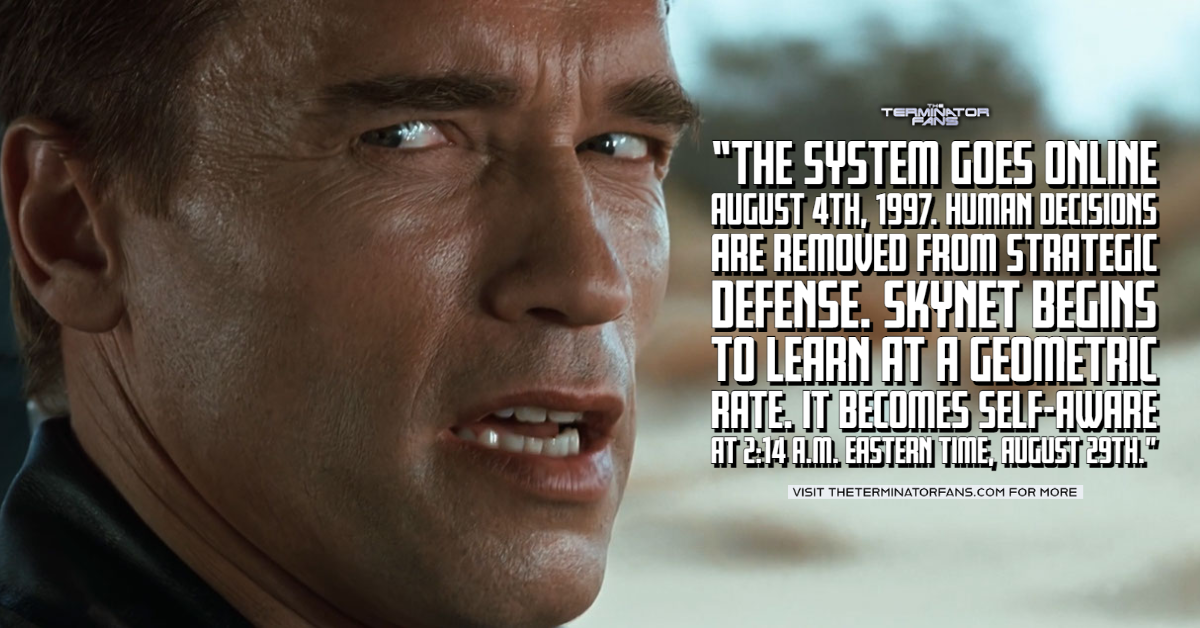
\includegraphics[width=\textwidth]{images/skynet.png}
\end{center}

\end{frame}

\begin{frame}
\frametitle{Reaction 2}

\begin{center}
	
\includegraphics[width=0.5\textwidth]{images/startup.jpg}
\end{center}

\end{frame}

\begin{frame}
\frametitle{Reaction 3}

\begin{center}
	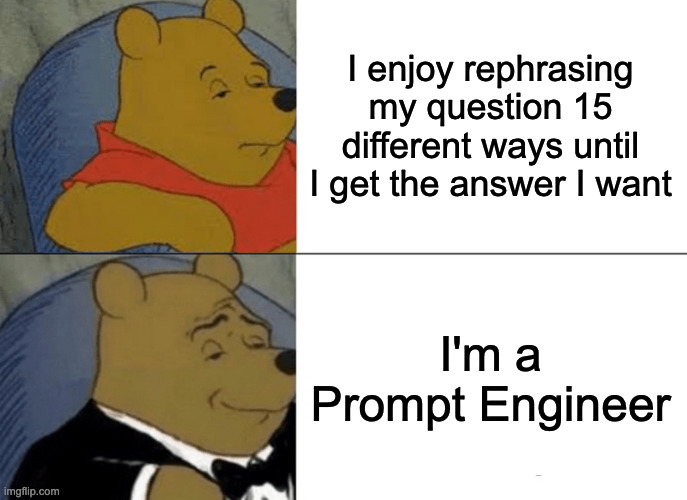
\includegraphics[width=0.75\textwidth]{images/prompt.jpg}
\end{center}

\end{frame}

\begin{frame}
\frametitle{Reaction 4}

\begin{center}
	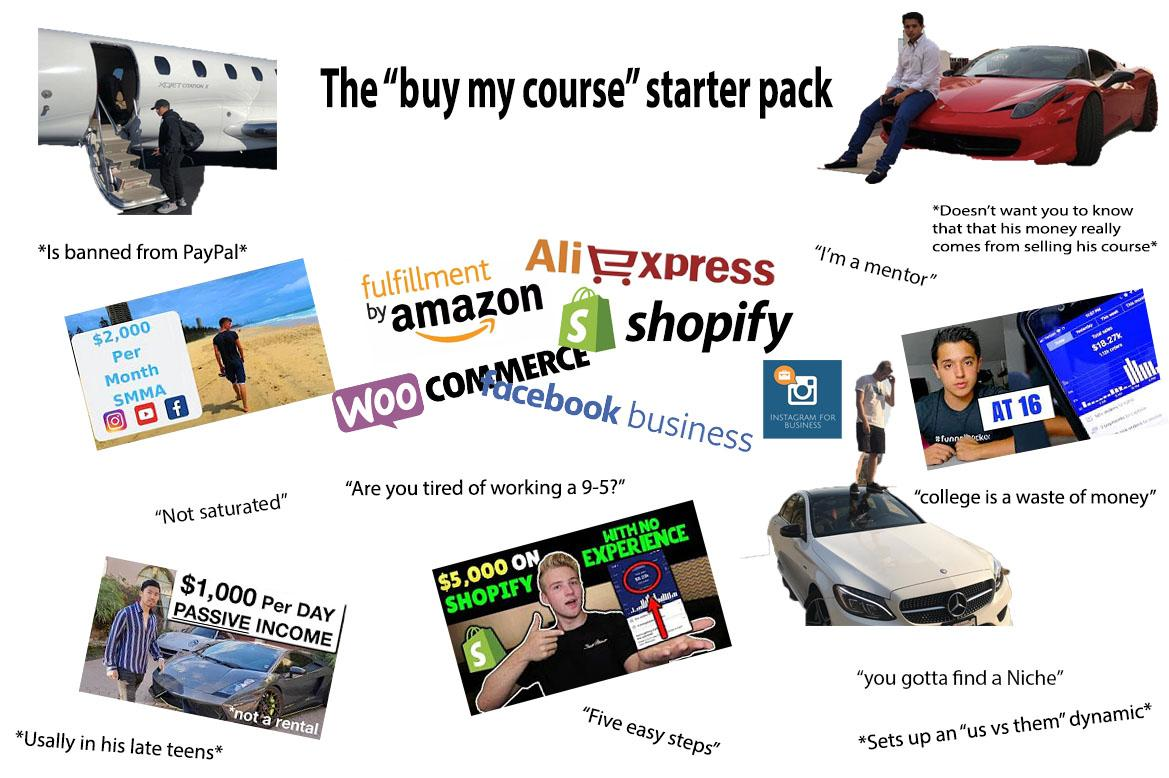
\includegraphics[width=0.75\textwidth]{images/starterpack.jpg}
\end{center}

\end{frame}


\begin{frame}
\frametitle{ChatGPT}

Such large language models have existed before, but ChatGPT ended up a hit because it's pretty good at being ``conversational''.

This is referred to as Natural Language Processing (NLP).

\end{frame}

\begin{frame}
\frametitle{ChatGPT}

Just because it gives you an answer, doesn't mean the answer is correct or true.

\begin{center}
	
\includegraphics[width=0.4\textwidth]{images/le-failed.jpg}
\end{center}

AI is subject to \alert{hallucinations}.

\end{frame}

\begin{frame}
\frametitle{Remember, The Law...}
Legally and professionally, the engineer is responsible for understanding how a given tool works \& verifying the output is reasonable \& correct.

\begin{center}
	
\includegraphics[width=0.5\textwidth]{images/jail.jpg}
\end{center}

\end{frame}

\begin{frame}
\frametitle{Prepared in Advance?}
Part of what makes the GPT-3 and GPT-4 models better at producing output that matches our expectations is that it relies on pre-training.

This course is not one on neural networks, large language models, AI, or similar.

But performance is relevant here!

\end{frame}

\begin{frame}
\frametitle{Parameters}

One factor that matters in how good a model is: parameters.

Bigger is \textit{usually} better...\\
\quad But requires more computational and memory resources.

We can maybe tune some options!

\end{frame}

\begin{frame}
\frametitle{Let's Try Some Optimization}

This section is based on a guide from ``Hugging Face''. 

\begin{center}
	
\includegraphics[width=0.5\textwidth]{images/hugging-face.png}
\end{center}

You may have guessed by the placement of this topic in the course material that the GPU is the right choice for how to generate or train a large language model. 

\end{frame}

\begin{frame}
\frametitle{About that Name}

Just... uh... don't confuse Hugging Face with Facehugger...

\begin{center}
	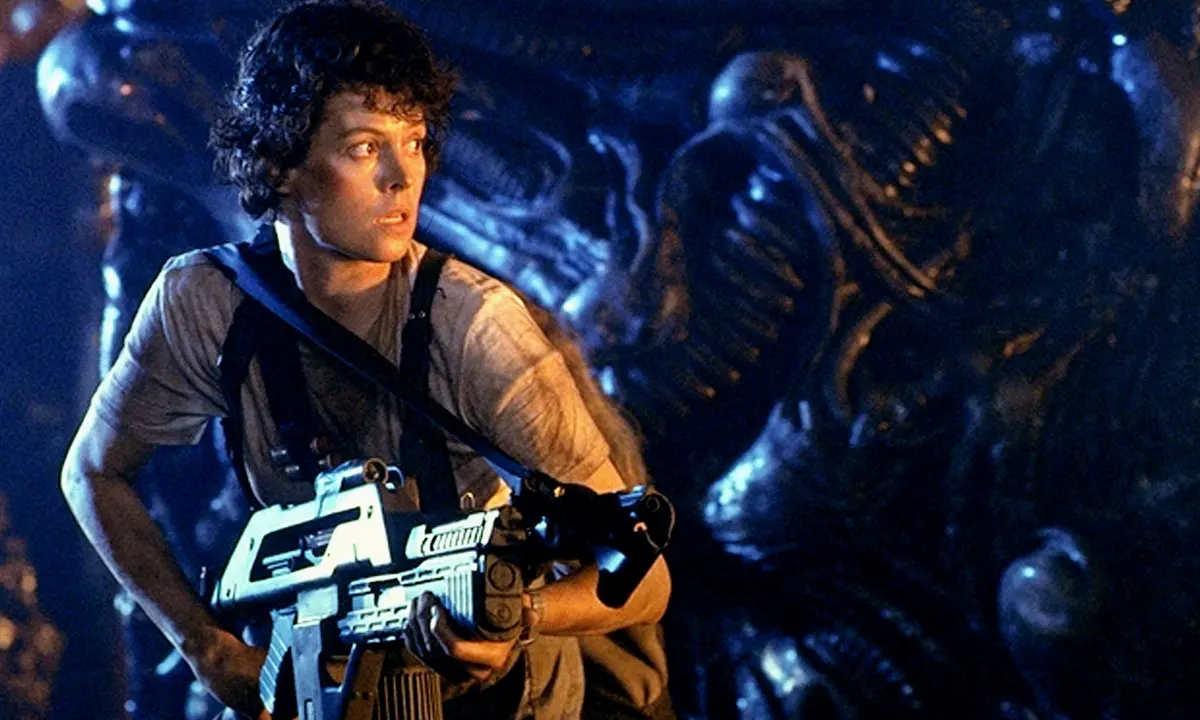
\includegraphics[width=0.75\textwidth]{images/ripley.jpg}
\end{center}

\end{frame}

\begin{frame}
\frametitle{Why a GPU?}

In this case we're talking about Transformers.

There are three main groups of optimizations that it does:\\
\begin{itemize} 
	\item Tensor Contractions
	\item Statistical Normalizations
	\item Element-Wise Operators
\end{itemize}

We also need to consider what's in memory.

\end{frame}

\begin{frame}
\frametitle{Optimize What?}

We can focus on how to generate a model that gives answers quickly...

Or we can focus on how to generate or train the model quickly.

\end{frame}

\begin{frame}
\frametitle{Make a Fast Model}

Use more space to reduce CPU usage, optimize for common cases, speculate...

Some of these are more fun than others: given a particular question, can you guess what the followup might be? 

\begin{center}
	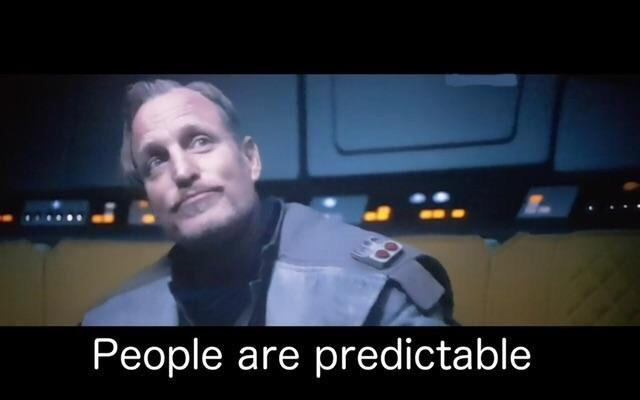
\includegraphics[width=0.5\textwidth]{images/predictable.jpg}
\end{center}

\end{frame}

\begin{frame}
\frametitle{Make a Model Fast}

Why would we customize some LLM?

Don't send your data to OpenAI...

Specialize for your workload.

\end{frame}

\begin{frame}
\frametitle{Batch Size}

Our first major optimization, and perhaps the easiest to do, is the batch size.

\begin{center}
	
\includegraphics[width=0.3\textwidth]{images/badbatch.jpg}
\end{center}


\end{frame}

\begin{frame}
\frametitle{Let's Review the Code}

The code is a little too large for the slides so let's go over it in a code editor.


The bert-large-uncased model is about 340~MB.

It's uncased because it makes no distinction between capitals and lower-case letters, e.g., it sees ``Word'' and ``word'' as equivalent.

\end{frame}

\begin{frame}[fragile]
\frametitle{Let's Try Training}

{\scriptsize
\begin{verbatim}
jzarnett@ecetesla0:~/github/ece459/lectures/live-coding/L24$ python3 dummy_data.py 
Starting up. Initial GPU utilization:
GPU memory occupied: 0 MB.
Initialized Torch; current GPU utilization:
GPU memory occupied: 417 MB.
Some weights of BertForSequenceClassification were not initialized 
from the model checkpoint at  bert-large-uncased and are newly initialized: 
['classifier.bias', 'classifier.weight']
You should probably TRAIN this model on a down-stream task to be able 
to use it for predictions and inference.
GPU memory occupied: 1705 MB.
torch.cuda.OutOfMemoryError: CUDA out of memory. Tried to allocate 20.00 MiB (GPU 0; 
7.43 GiB total capacity; 6.90 GiB already allocated; 16.81 MiB free; 6.90 GiB 
reserved in total by PyTorch) If reserved memory is >> allocated memory try setting 
max_split_size_mb to avoid fragmentation.  See documentation for Memory Management
and PYTORCH_CUDA_ALLOC_CONF
\end{verbatim}
}

\end{frame}

\begin{frame}[fragile]
\frametitle{Let's See the Problem}
I asked \texttt{nvidia-smi}...

{\scriptsize
\begin{verbatim}
+-----------------------------------------------------------------------------+
| NVIDIA-SMI 470.199.02   Driver Version: 470.199.02   CUDA Version: 11.4     |
|-------------------------------+----------------------+----------------------+
| GPU  Name        Persistence-M| Bus-Id        Disp.A | Volatile Uncorr. ECC |
| Fan  Temp  Perf  Pwr:Usage/Cap|         Memory-Usage | GPU-Util  Compute M. |
|                               |                      |               MIG M. |
|===============================+======================+======================|
|   0  Tesla P4            Off  | 00000000:17:00.0 Off |                    0 |
| N/A   42C    P0    23W /  75W |      0MiB /  7611MiB |      1%      Default |
|                               |                      |                  N/A |
+-------------------------------+----------------------+----------------------+
                                                                               
+-----------------------------------------------------------------------------+
| Processes:                                                                  |
|  GPU   GI   CI        PID   Type   Process name                  GPU Memory |
|        ID   ID                                                   Usage      |
|=============================================================================|
|  No running processes found                                                 |
+-----------------------------------------------------------------------------+
\end{verbatim}
}


\end{frame}

\begin{frame}
\frametitle{Kirk to Engineering...}

7~611 MB is not enough for this model...

\begin{center}
	
\includegraphics[width=0.5\textwidth]{images/morepower.png}
\end{center}

Problem is we don't have any bigger VRAM cards.

\end{frame}

\begin{frame}
\frametitle{Fine, I Guess}

What I actually did next was change to a smaller version of the model, \texttt{bert-base-uncased}.

It's significantly smaller (110~MB) and something the card could handle. 

\end{frame}

\begin{frame}[fragile]
\frametitle{Smaller Model Output}

{\scriptsize
\begin{verbatim}
jzarnett@ecetesla0:~/github/ece459/lectures/live-coding/L24$ python3 dummy_data.py 
Starting up. Initial GPU utilization:
GPU memory occupied: 0 MB.
Initialized Torch; current GPU utilization:
GPU memory occupied: 417 MB.
Some weights of BertForSequenceClassification were not initialized from the 
model checkpoint at  bert-base-uncased and are newly initialized: 
['classifier.weight', 'classifier.bias']
You should probably TRAIN this model on a down-stream task to be able to use
 it for predictions and inference.
GPU memory occupied: 887 MB.
{'loss': 0.0028, 'learning_rate': 1.1718750000000001e-06, 'epoch': 0.98}
{'train_runtime': 109.6152, 'train_samples_per_second': 4.671, 
'train_steps_per_second': 4.671, 'train_loss': 0.0027378778694355788, 'epoch': 1.0}
Time: 109.62
Samples/second: 4.67
GPU memory occupied: 3281 MB.
\end{verbatim}
}

\end{frame}

\begin{frame}
\frametitle{Results Table}

Then I needed to experiment some more with batch size to find the ideal.

\begin{center}
\begin{tabular}{r|r|r|r|r}
\textbf{Batch Size} & \textbf{Time (s)} & \textbf{Samples/s} & \textbf{Memory Used (MB)} & \textbf{Utilization (\%)} \\ \hline
1 & 109.62 & 4.67 & 3~281 & 43.1 \\
2 & 85.82 & 5.97 & 3~391 & 44.6 \\
4 & 72.18 & 7.09 & 4~613 & 60.6 \\
8 & 66.70 & 7.68 & 7~069 & 92.9 \\
\end{tabular}
\end{center}

Unsurprisingly, choosing batch size of 9 leads to OOM.

\end{frame}

\begin{frame}
\frametitle{Next Idea}

We seem to be memory limited -- let's see what we can do?

First idea: \alert{gradient accumulation}. 

Calculate gradients in small increments rather than for the whole batch.

\end{frame}

\begin{frame}
\frametitle{Experimenting with Gradient Accumulation}

\begin{center}
\begin{tabular}{r|r|r|r|r}
\textbf{Steps} & \textbf{Time (s)} & \textbf{Samples/s} & \textbf{Memory Used (MB)} & \textbf{Utilization (\%)} \\ \hline
1 & 66.06 & 7.75 & 7~069 & 92.9 \\
2 & 63.96 & 8.01 & 7~509 & 98.7 \\
4 & 62.81 & 8.15 & 7~509 & 98.7 \\
8 & 62.65 & 8.17 & 7~509 & 98.7 \\
16 & 62.42 & 8.20 & 7~509 & 98.7 \\
32 & 62.44 & 8.20 & 7~509 & 98.7\\
128 & 62.20 & 8.23 & 6~637 & 87.2\\
1024 & 61.78 & 8.29 & 6~637 & 87.2 \\
4096 & 62.16 & 8.24 & 6~637 & 87.2
\end{tabular}
\end{center}

\end{frame}

\begin{frame}
\frametitle{I got Suspicious}

I got suspicious about the 128 dropoff in memory usage and it made me think about other indicators -- is it getting worse somehow? 

The output talks about training loss...

\begin{center}
\begin{tabular}{r|r}
\textbf{Gradient Accumulation Steps} & \textbf{Loss} \\ \hline
1 & 0.029 \\
2 & 0.070 \\
4 & 0.163 \\
8 & 0.169 \\
16 & 0.447 \\
32 & 0.445 \\
128 & 0.435 \\
1024 & 0.463 \\
4096 & 0.014 \\
\end{tabular}
\end{center}

Is that concerning?

\end{frame}

\begin{frame}
\frametitle{Let's Validate}

We need to do some validation of how it's going...


We'll train and validate using some Yelp data.

\begin{center}
	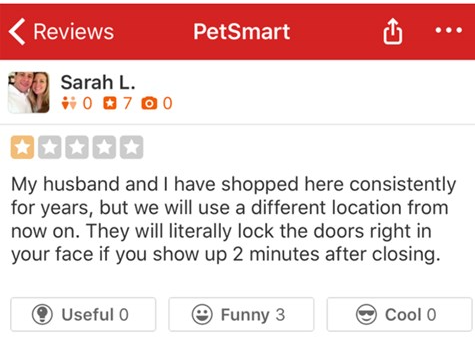
\includegraphics[width=0.6\textwidth]{images/yelp.png}
\end{center}

\end{frame}

\begin{frame}
\frametitle{More Code, More Review}

The python code here is significantly different but we'll take a look.

I've skipped some intermediate results since at 9 minutes to calculate it takes a while to fill in all the values above.


\end{frame}

\begin{frame}
\frametitle{Accuracy Results}

\begin{center}
\begin{tabular}{r|r|r|r|r}
\textbf{GA Steps} & \textbf{Time (s)} & \textbf{Samples/s} & \textbf{Memory Used (MB)} & \textbf{Final Accuracy}\\ \hline
1 & 538.37 & 5.56 & 7~069 & 0.621 \\
8 & 501.89 & 5.98 & 7~509 & 0.554 \\
32 & 429.70 & 6.98 & 7~509 & 0.347 \\
1024 & 513.17 & 5.85 & 7~509 & 0.222 \\
\end{tabular}
\end{center}

Interesting results -- maybe a little concerning?

\end{frame}

\begin{frame}
\frametitle{More Isn't Always Better}

Increasing the gradient accumulation does change the effective batch size...

Batch size too large may mean less ability to generalize (overfitting).

But smaller isn't always better either; can underfit the data.

In the Yelp example, I get worse accuracy with batch size of 1 than 4, and 4 is worse than 8. There really is no magic number.


\end{frame}

\begin{frame}
\frametitle{Gradient Checkpointing}

\alert{Gradient Checkpointing}: increase compute time to save memory.

Instead of saving activations, save only some, recompute the rest.

Does it work?

\end{frame}

\begin{frame}
\frametitle{Gradient Checkpointing}

Trying this out with batch size of 8, the total time goes from 66.70 to 93.07s and the memory from 7~069 down to 3~619 MB. 

As expected, we got slower but used less memory. 

Maybe it means we can increase the batch size? 

Raising it to 16 means the time was  100.55s but still only 3~731 MB


\end{frame}

\begin{frame}
\frametitle{Gradient Checkpointing}

Increasing the batch size a lot to finish faster might work eventually. 

And no, using this checkpointing even with a batch size of 1 is not sufficient to run the \texttt{bert-large-uncased} model on \texttt{ecetesla0}.

And remember that excessively large batch sizes aren't good...

\end{frame}

\begin{frame}
\frametitle{Mixed Precision, Data Preloading}

\alert{Mixed Precision}: Use less accurate types (16 vs 32-bit).

\alert{Data Preloading}: Multithread to get data to GPU faster.

Other ideas: Mixture of Experts, bigger GPU, multiple-GPU...

\end{frame}

\begin{frame}
\frametitle{Tradeoffs}
\begin{multicols}{2}

\includegraphics[width=0.35\textwidth]{images/tradeoffer.jpg}
\columnbreak
\begin{itemize}
\item Accuracy for time? \\[5em]

\item Memory for CPU? \\[5em]

\item Err on the side of over- or under-fitting?
\end{itemize}
\end{multicols}

\end{frame}

\begin{frame}
\frametitle{Tradeoffs}

In the next few years, technologies and decision-making for this will become much more sophisticated.

But in the meantime, we can have a lot of fun experimenting and learning.
\begin{center}
	
\includegraphics[width=0.4\textwidth]{images/funbegins.jpg}
\end{center}




\end{frame}


\end{document}
